% Created by tikzDevice version 0.10.1 on 2018-01-31 09:59:17
% !TEX encoding = UTF-8 Unicode
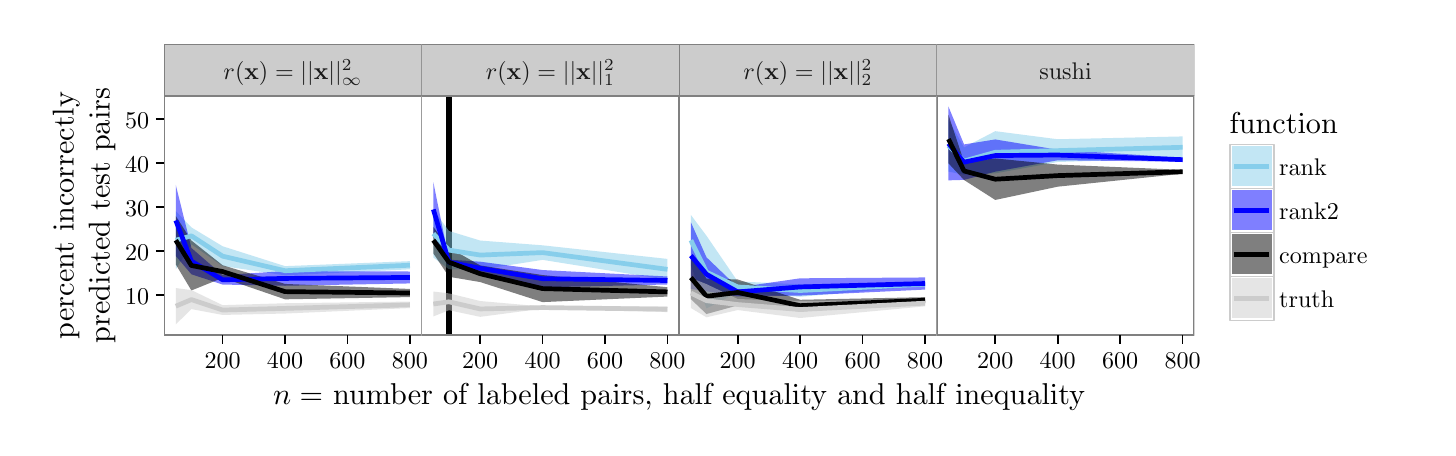
\begin{tikzpicture}[x=1pt,y=1pt]
\definecolor{fillColor}{RGB}{255,255,255}
\path[use as bounding box,fill=fillColor,fill opacity=0.00] (0,0) rectangle (505.89,144.54);
\begin{scope}
\path[clip] (  0.00,  0.00) rectangle (505.89,144.54);
\definecolor{drawColor}{RGB}{255,255,255}
\definecolor{fillColor}{RGB}{255,255,255}

\path[draw=drawColor,line width= 0.6pt,line join=round,line cap=round,fill=fillColor] ( -0.00, -0.00) rectangle (505.89,144.54);
\end{scope}
\begin{scope}
\path[clip] ( 49.29,119.96) rectangle (142.36,138.54);
\definecolor{drawColor}{gray}{0.50}
\definecolor{fillColor}{gray}{0.80}

\path[draw=drawColor,line width= 0.2pt,line join=round,line cap=round,fill=fillColor] ( 49.29,119.96) rectangle (142.36,138.54);
\definecolor{drawColor}{gray}{0.10}

\node[text=drawColor,anchor=base,inner sep=0pt, outer sep=0pt, scale=  0.87] at ( 95.82,125.96) {$r(\mathbf x) = ||\mathbf x||_\infty^2$};
\end{scope}
\begin{scope}
\path[clip] (142.36,119.96) rectangle (235.42,138.54);
\definecolor{drawColor}{gray}{0.50}
\definecolor{fillColor}{gray}{0.80}

\path[draw=drawColor,line width= 0.2pt,line join=round,line cap=round,fill=fillColor] (142.36,119.96) rectangle (235.42,138.54);
\definecolor{drawColor}{gray}{0.10}

\node[text=drawColor,anchor=base,inner sep=0pt, outer sep=0pt, scale=  0.87] at (188.89,125.96) {$r(\mathbf x) = ||\mathbf x||_1^2$};
\end{scope}
\begin{scope}
\path[clip] (235.42,119.96) rectangle (328.49,138.54);
\definecolor{drawColor}{gray}{0.50}
\definecolor{fillColor}{gray}{0.80}

\path[draw=drawColor,line width= 0.2pt,line join=round,line cap=round,fill=fillColor] (235.42,119.96) rectangle (328.49,138.54);
\definecolor{drawColor}{gray}{0.10}

\node[text=drawColor,anchor=base,inner sep=0pt, outer sep=0pt, scale=  0.87] at (281.96,125.96) {$r(\mathbf x) = ||\mathbf x||_2^2$};
\end{scope}
\begin{scope}
\path[clip] (328.49,119.96) rectangle (421.56,138.54);
\definecolor{drawColor}{gray}{0.50}
\definecolor{fillColor}{gray}{0.80}

\path[draw=drawColor,line width= 0.2pt,line join=round,line cap=round,fill=fillColor] (328.49,119.96) rectangle (421.56,138.54);
\definecolor{drawColor}{gray}{0.10}

\node[text=drawColor,anchor=base,inner sep=0pt, outer sep=0pt, scale=  0.87] at (375.02,125.96) {sushi};
\end{scope}
\begin{scope}
\path[clip] ( 49.29, 33.41) rectangle (142.36,119.96);
\definecolor{fillColor}{RGB}{255,255,255}

\path[fill=fillColor] ( 49.29, 33.41) rectangle (142.36,119.96);
\definecolor{fillColor}{RGB}{135,206,235}

\path[fill=fillColor,fill opacity=0.50] ( 53.52, 78.24) --
	( 59.16, 72.37) --
	( 70.44, 65.55) --
	( 93.00, 58.37) --
	(138.13, 60.17) --
	(138.13, 57.22) --
	( 93.00, 55.04) --
	( 70.44, 58.40) --
	( 59.16, 66.28) --
	( 53.52, 57.23) --
	cycle;
\definecolor{fillColor}{RGB}{0,0,255}

\path[fill=fillColor,fill opacity=0.50] ( 53.52, 87.73) --
	( 59.16, 64.93) --
	( 70.44, 55.15) --
	( 93.00, 56.57) --
	(138.13, 56.43) --
	(138.13, 52.12) --
	( 93.00, 51.28) --
	( 70.44, 51.71) --
	( 59.16, 55.44) --
	( 53.52, 62.04) --
	cycle;
\definecolor{fillColor}{RGB}{0,0,0}

\path[fill=fillColor,fill opacity=0.50] ( 53.52, 76.49) --
	( 59.16, 67.62) --
	( 70.44, 58.69) --
	( 93.00, 51.94) --
	(138.13, 50.13) --
	(138.13, 47.19) --
	( 93.00, 46.38) --
	( 70.44, 54.13) --
	( 59.16, 49.57) --
	( 53.52, 58.98) --
	cycle;
\definecolor{fillColor}{RGB}{204,204,204}

\path[fill=fillColor,fill opacity=0.50] ( 53.52, 50.45) --
	( 59.16, 49.71) --
	( 70.44, 44.27) --
	( 93.00, 44.96) --
	(138.13, 45.57) --
	(138.13, 43.22) --
	( 93.00, 41.24) --
	( 70.44, 40.74) --
	( 59.16, 42.85) --
	( 53.52, 37.34) --
	cycle;
\definecolor{drawColor}{RGB}{135,206,235}

\path[draw=drawColor,line width= 1.7pt,line join=round] ( 53.52, 67.73) --
	( 59.16, 69.32) --
	( 70.44, 61.97) --
	( 93.00, 56.71) --
	(138.13, 58.70);
\definecolor{drawColor}{RGB}{0,0,255}

\path[draw=drawColor,line width= 1.7pt,line join=round] ( 53.52, 74.89) --
	( 59.16, 60.19) --
	( 70.44, 53.43) --
	( 93.00, 53.93) --
	(138.13, 54.28);
\definecolor{drawColor}{RGB}{0,0,0}

\path[draw=drawColor,line width= 1.7pt,line join=round] ( 53.52, 67.73) --
	( 59.16, 58.60) --
	( 70.44, 56.41) --
	( 93.00, 49.16) --
	(138.13, 48.66);
\definecolor{drawColor}{gray}{0.80}

\path[draw=drawColor,line width= 1.7pt,line join=round] ( 53.52, 43.90) --
	( 59.16, 46.28) --
	( 70.44, 42.51) --
	( 93.00, 43.10) --
	(138.13, 44.39);
\definecolor{drawColor}{gray}{0.50}

\path[draw=drawColor,line width= 0.6pt,line join=round,line cap=round] ( 49.29, 33.41) rectangle (142.36,119.96);
\end{scope}
\begin{scope}
\path[clip] (142.36, 33.41) rectangle (235.42,119.96);
\definecolor{fillColor}{RGB}{255,255,255}

\path[fill=fillColor] (142.36, 33.41) rectangle (235.42,119.96);
\definecolor{drawColor}{RGB}{0,0,0}

\path[draw=drawColor,line width= 2.3pt,line join=round] (152.23, 33.41) -- (152.23,119.96);
\definecolor{fillColor}{RGB}{135,206,235}

\path[fill=fillColor,fill opacity=0.50] (146.59, 78.72) --
	(152.23, 71.07) --
	(163.51, 67.62) --
	(186.07, 65.89) --
	(231.19, 60.98) --
	(231.19, 53.43) --
	(186.07, 60.64) --
	(163.51, 57.12) --
	(152.23, 57.25) --
	(146.59, 61.51) --
	cycle;
\definecolor{fillColor}{RGB}{0,0,255}

\path[fill=fillColor,fill opacity=0.50] (146.59, 88.70) --
	(152.23, 60.71) --
	(163.51, 59.98) --
	(186.07, 56.96) --
	(231.19, 54.63) --
	(231.19, 51.74) --
	(186.07, 50.70) --
	(163.51, 55.23) --
	(152.23, 58.87) --
	(146.59, 69.02) --
	cycle;
\definecolor{fillColor}{RGB}{0,0,0}

\path[fill=fillColor,fill opacity=0.50] (146.59, 72.50) --
	(152.23, 65.06) --
	(163.51, 58.62) --
	(186.07, 55.14) --
	(231.19, 50.75) --
	(231.19, 47.37) --
	(186.07, 45.37) --
	(163.51, 52.62) --
	(152.23, 54.52) --
	(146.59, 62.97) --
	cycle;
\definecolor{fillColor}{RGB}{204,204,204}

\path[fill=fillColor,fill opacity=0.50] (146.59, 49.19) --
	(152.23, 48.53) --
	(163.51, 45.76) --
	(186.07, 43.78) --
	(231.19, 43.84) --
	(231.19, 41.77) --
	(186.07, 43.02) --
	(163.51, 40.05) --
	(152.23, 42.44) --
	(146.59, 40.20) --
	cycle;
\definecolor{drawColor}{RGB}{135,206,235}

\path[draw=drawColor,line width= 1.7pt,line join=round] (146.59, 70.12) --
	(152.23, 64.16) --
	(163.51, 62.37) --
	(186.07, 63.26) --
	(231.19, 57.21);
\definecolor{drawColor}{RGB}{0,0,255}

\path[draw=drawColor,line width= 1.7pt,line join=round] (146.59, 78.86) --
	(152.23, 59.79) --
	(163.51, 57.60) --
	(186.07, 53.83) --
	(231.19, 53.18);
\definecolor{drawColor}{RGB}{0,0,0}

\path[draw=drawColor,line width= 1.7pt,line join=round] (146.59, 67.73) --
	(152.23, 59.79) --
	(163.51, 55.62) --
	(186.07, 50.25) --
	(231.19, 49.06);
\definecolor{drawColor}{gray}{0.80}

\path[draw=drawColor,line width= 1.7pt,line join=round] (146.59, 44.69) --
	(152.23, 45.48) --
	(163.51, 42.90) --
	(186.07, 43.40) --
	(231.19, 42.80);
\definecolor{drawColor}{gray}{0.50}

\path[draw=drawColor,line width= 0.6pt,line join=round,line cap=round] (142.36, 33.41) rectangle (235.42,119.96);
\end{scope}
\begin{scope}
\path[clip] (235.42, 33.41) rectangle (328.49,119.96);
\definecolor{fillColor}{RGB}{255,255,255}

\path[fill=fillColor] (235.42, 33.41) rectangle (328.49,119.96);
\definecolor{fillColor}{RGB}{135,206,235}

\path[fill=fillColor,fill opacity=0.50] (239.65, 76.86) --
	(245.29, 69.34) --
	(256.57, 52.84) --
	(279.14, 51.81) --
	(324.26, 52.40) --
	(324.26, 51.28) --
	(279.14, 47.30) --
	(256.57, 48.86) --
	(245.29, 43.08) --
	(239.65, 58.60) --
	cycle;
\definecolor{fillColor}{RGB}{0,0,255}

\path[fill=fillColor,fill opacity=0.50] (239.65, 74.21) --
	(245.29, 61.56) --
	(256.57, 50.71) --
	(279.14, 53.97) --
	(324.26, 54.28) --
	(324.26, 49.90) --
	(279.14, 47.73) --
	(256.57, 47.41) --
	(245.29, 49.28) --
	(239.65, 50.14) --
	cycle;
\definecolor{fillColor}{RGB}{0,0,0}

\path[fill=fillColor,fill opacity=0.50] (239.65, 62.01) --
	(245.29, 53.88) --
	(256.57, 53.56) --
	(279.14, 46.21) --
	(324.26, 47.16) --
	(324.26, 44.90) --
	(279.14, 41.98) --
	(256.57, 44.17) --
	(245.29, 41.07) --
	(239.65, 46.44) --
	cycle;
\definecolor{fillColor}{RGB}{204,204,204}

\path[fill=fillColor,fill opacity=0.50] (239.65, 54.09) --
	(245.29, 51.88) --
	(256.57, 46.48) --
	(279.14, 45.78) --
	(324.26, 46.13) --
	(324.26, 43.85) --
	(279.14, 39.63) --
	(256.57, 42.51) --
	(245.29, 39.88) --
	(239.65, 43.24) --
	cycle;
\definecolor{drawColor}{RGB}{135,206,235}

\path[draw=drawColor,line width= 1.7pt,line join=round] (239.65, 67.73) --
	(245.29, 56.21) --
	(256.57, 50.85) --
	(279.14, 49.56) --
	(324.26, 51.84);
\definecolor{drawColor}{RGB}{0,0,255}

\path[draw=drawColor,line width= 1.7pt,line join=round] (239.65, 62.17) --
	(245.29, 55.42) --
	(256.57, 49.06) --
	(279.14, 50.85) --
	(324.26, 52.09);
\definecolor{drawColor}{RGB}{0,0,0}

\path[draw=drawColor,line width= 1.7pt,line join=round] (239.65, 54.23) --
	(245.29, 47.47) --
	(256.57, 48.86) --
	(279.14, 44.09) --
	(324.26, 46.03);
\definecolor{drawColor}{gray}{0.80}

\path[draw=drawColor,line width= 1.7pt,line join=round] (239.65, 48.66) --
	(245.29, 45.88) --
	(256.57, 44.49) --
	(279.14, 42.70) --
	(324.26, 44.99);
\definecolor{drawColor}{gray}{0.50}

\path[draw=drawColor,line width= 0.6pt,line join=round,line cap=round] (235.42, 33.41) rectangle (328.49,119.96);
\end{scope}
\begin{scope}
\path[clip] (328.49, 33.41) rectangle (421.56,119.96);
\definecolor{fillColor}{RGB}{255,255,255}

\path[fill=fillColor] (328.49, 33.41) rectangle (421.56,119.96);
\definecolor{fillColor}{RGB}{135,206,235}

\path[fill=fillColor,fill opacity=0.50] (332.72,111.26) --
	(338.36,101.28) --
	(349.64,107.14) --
	(372.20,104.22) --
	(417.33,105.24) --
	(417.33, 97.37) --
	(372.20, 96.00) --
	(349.64, 91.90) --
	(338.36, 91.40) --
	(332.72, 92.54) --
	cycle;
\definecolor{fillColor}{RGB}{0,0,255}

\path[fill=fillColor,fill opacity=0.50] (332.72,116.02) --
	(338.36,102.35) --
	(349.64,104.15) --
	(372.20,100.43) --
	(417.33, 97.54) --
	(417.33, 96.13) --
	(372.20, 96.62) --
	(349.64, 92.51) --
	(338.36, 89.54) --
	(332.72, 89.37) --
	cycle;
\definecolor{fillColor}{RGB}{0,0,0}

\path[fill=fillColor,fill opacity=0.50] (332.72,113.04) --
	(338.36, 96.04) --
	(349.64, 97.28) --
	(372.20, 95.07) --
	(417.33, 93.17) --
	(417.33, 91.76) --
	(372.20, 87.08) --
	(349.64, 82.29) --
	(338.36, 89.49) --
	(332.72, 95.53) --
	cycle;
\definecolor{drawColor}{RGB}{135,206,235}

\path[draw=drawColor,line width= 1.7pt,line join=round] (332.72,101.90) --
	(338.36, 96.34) --
	(349.64, 99.52) --
	(372.20,100.11) --
	(417.33,101.31);
\definecolor{drawColor}{RGB}{0,0,255}

\path[draw=drawColor,line width= 1.7pt,line join=round] (332.72,102.70) --
	(338.36, 95.94) --
	(349.64, 98.33) --
	(372.20, 98.52) --
	(417.33, 96.84);
\definecolor{drawColor}{RGB}{0,0,0}

\path[draw=drawColor,line width= 1.7pt,line join=round] (332.72,104.29) --
	(338.36, 92.76) --
	(349.64, 89.78) --
	(372.20, 91.08) --
	(417.33, 92.47);
\definecolor{drawColor}{gray}{0.50}

\path[draw=drawColor,line width= 0.6pt,line join=round,line cap=round] (328.49, 33.41) rectangle (421.56,119.96);
\end{scope}
\begin{scope}
\path[clip] (  0.00,  0.00) rectangle (505.89,144.54);
\definecolor{drawColor}{RGB}{0,0,0}

\node[text=drawColor,anchor=base east,inner sep=0pt, outer sep=0pt, scale=  0.87] at ( 43.89, 44.58) {10};

\node[text=drawColor,anchor=base east,inner sep=0pt, outer sep=0pt, scale=  0.87] at ( 43.89, 60.47) {20};

\node[text=drawColor,anchor=base east,inner sep=0pt, outer sep=0pt, scale=  0.87] at ( 43.89, 76.36) {30};

\node[text=drawColor,anchor=base east,inner sep=0pt, outer sep=0pt, scale=  0.87] at ( 43.89, 92.25) {40};

\node[text=drawColor,anchor=base east,inner sep=0pt, outer sep=0pt, scale=  0.87] at ( 43.89,108.15) {50};
\end{scope}
\begin{scope}
\path[clip] (  0.00,  0.00) rectangle (505.89,144.54);
\definecolor{drawColor}{RGB}{0,0,0}

\path[draw=drawColor,line width= 0.6pt,line join=round] ( 46.29, 47.87) --
	( 49.29, 47.87);

\path[draw=drawColor,line width= 0.6pt,line join=round] ( 46.29, 63.76) --
	( 49.29, 63.76);

\path[draw=drawColor,line width= 0.6pt,line join=round] ( 46.29, 79.65) --
	( 49.29, 79.65);

\path[draw=drawColor,line width= 0.6pt,line join=round] ( 46.29, 95.55) --
	( 49.29, 95.55);

\path[draw=drawColor,line width= 0.6pt,line join=round] ( 46.29,111.44) --
	( 49.29,111.44);
\end{scope}
\begin{scope}
\path[clip] (  0.00,  0.00) rectangle (505.89,144.54);
\definecolor{drawColor}{RGB}{0,0,0}

\path[draw=drawColor,line width= 0.6pt,line join=round] ( 70.44, 30.41) --
	( 70.44, 33.41);

\path[draw=drawColor,line width= 0.6pt,line join=round] ( 93.00, 30.41) --
	( 93.00, 33.41);

\path[draw=drawColor,line width= 0.6pt,line join=round] (115.56, 30.41) --
	(115.56, 33.41);

\path[draw=drawColor,line width= 0.6pt,line join=round] (138.13, 30.41) --
	(138.13, 33.41);
\end{scope}
\begin{scope}
\path[clip] (  0.00,  0.00) rectangle (505.89,144.54);
\definecolor{drawColor}{RGB}{0,0,0}

\node[text=drawColor,anchor=base,inner sep=0pt, outer sep=0pt, scale=  0.87] at ( 70.44, 21.43) {200};

\node[text=drawColor,anchor=base,inner sep=0pt, outer sep=0pt, scale=  0.87] at ( 93.00, 21.43) {400};

\node[text=drawColor,anchor=base,inner sep=0pt, outer sep=0pt, scale=  0.87] at (115.56, 21.43) {600};

\node[text=drawColor,anchor=base,inner sep=0pt, outer sep=0pt, scale=  0.87] at (138.13, 21.43) {800};
\end{scope}
\begin{scope}
\path[clip] (  0.00,  0.00) rectangle (505.89,144.54);
\definecolor{drawColor}{RGB}{0,0,0}

\path[draw=drawColor,line width= 0.6pt,line join=round] (163.51, 30.41) --
	(163.51, 33.41);

\path[draw=drawColor,line width= 0.6pt,line join=round] (186.07, 30.41) --
	(186.07, 33.41);

\path[draw=drawColor,line width= 0.6pt,line join=round] (208.63, 30.41) --
	(208.63, 33.41);

\path[draw=drawColor,line width= 0.6pt,line join=round] (231.19, 30.41) --
	(231.19, 33.41);
\end{scope}
\begin{scope}
\path[clip] (  0.00,  0.00) rectangle (505.89,144.54);
\definecolor{drawColor}{RGB}{0,0,0}

\node[text=drawColor,anchor=base,inner sep=0pt, outer sep=0pt, scale=  0.87] at (163.51, 21.43) {200};

\node[text=drawColor,anchor=base,inner sep=0pt, outer sep=0pt, scale=  0.87] at (186.07, 21.43) {400};

\node[text=drawColor,anchor=base,inner sep=0pt, outer sep=0pt, scale=  0.87] at (208.63, 21.43) {600};

\node[text=drawColor,anchor=base,inner sep=0pt, outer sep=0pt, scale=  0.87] at (231.19, 21.43) {800};
\end{scope}
\begin{scope}
\path[clip] (  0.00,  0.00) rectangle (505.89,144.54);
\definecolor{drawColor}{RGB}{0,0,0}

\path[draw=drawColor,line width= 0.6pt,line join=round] (256.57, 30.41) --
	(256.57, 33.41);

\path[draw=drawColor,line width= 0.6pt,line join=round] (279.14, 30.41) --
	(279.14, 33.41);

\path[draw=drawColor,line width= 0.6pt,line join=round] (301.70, 30.41) --
	(301.70, 33.41);

\path[draw=drawColor,line width= 0.6pt,line join=round] (324.26, 30.41) --
	(324.26, 33.41);
\end{scope}
\begin{scope}
\path[clip] (  0.00,  0.00) rectangle (505.89,144.54);
\definecolor{drawColor}{RGB}{0,0,0}

\node[text=drawColor,anchor=base,inner sep=0pt, outer sep=0pt, scale=  0.87] at (256.57, 21.43) {200};

\node[text=drawColor,anchor=base,inner sep=0pt, outer sep=0pt, scale=  0.87] at (279.14, 21.43) {400};

\node[text=drawColor,anchor=base,inner sep=0pt, outer sep=0pt, scale=  0.87] at (301.70, 21.43) {600};

\node[text=drawColor,anchor=base,inner sep=0pt, outer sep=0pt, scale=  0.87] at (324.26, 21.43) {800};
\end{scope}
\begin{scope}
\path[clip] (  0.00,  0.00) rectangle (505.89,144.54);
\definecolor{drawColor}{RGB}{0,0,0}

\path[draw=drawColor,line width= 0.6pt,line join=round] (349.64, 30.41) --
	(349.64, 33.41);

\path[draw=drawColor,line width= 0.6pt,line join=round] (372.20, 30.41) --
	(372.20, 33.41);

\path[draw=drawColor,line width= 0.6pt,line join=round] (394.76, 30.41) --
	(394.76, 33.41);

\path[draw=drawColor,line width= 0.6pt,line join=round] (417.33, 30.41) --
	(417.33, 33.41);
\end{scope}
\begin{scope}
\path[clip] (  0.00,  0.00) rectangle (505.89,144.54);
\definecolor{drawColor}{RGB}{0,0,0}

\node[text=drawColor,anchor=base,inner sep=0pt, outer sep=0pt, scale=  0.87] at (349.64, 21.43) {200};

\node[text=drawColor,anchor=base,inner sep=0pt, outer sep=0pt, scale=  0.87] at (372.20, 21.43) {400};

\node[text=drawColor,anchor=base,inner sep=0pt, outer sep=0pt, scale=  0.87] at (394.76, 21.43) {600};

\node[text=drawColor,anchor=base,inner sep=0pt, outer sep=0pt, scale=  0.87] at (417.33, 21.43) {800};
\end{scope}
\begin{scope}
\path[clip] (  0.00,  0.00) rectangle (505.89,144.54);
\definecolor{drawColor}{RGB}{0,0,0}

\node[text=drawColor,anchor=base,inner sep=0pt, outer sep=0pt, scale=  1.09] at (235.42,  8.40) {$n=$ number of labeled pairs, half equality and half inequality};
\end{scope}
\begin{scope}
\path[clip] (  0.00,  0.00) rectangle (505.89,144.54);
\definecolor{drawColor}{RGB}{0,0,0}

\node[text=drawColor,rotate= 90.00,anchor=base,inner sep=0pt, outer sep=0pt, scale=  1.09] at ( 16.63, 76.68) {percent incorrectly};

\node[text=drawColor,rotate= 90.00,anchor=base,inner sep=0pt, outer sep=0pt, scale=  1.09] at ( 29.59, 76.68) {predicted test pairs};
\end{scope}
\begin{scope}
\path[clip] (  0.00,  0.00) rectangle (505.89,144.54);
\definecolor{fillColor}{RGB}{255,255,255}

\path[fill=fillColor] (430.09, 34.52) rectangle (491.35,118.85);
\end{scope}
\begin{scope}
\path[clip] (  0.00,  0.00) rectangle (505.89,144.54);
\definecolor{drawColor}{RGB}{0,0,0}

\node[text=drawColor,anchor=base west,inner sep=0pt, outer sep=0pt, scale=  1.09] at (434.36,106.36) {function};
\end{scope}
\begin{scope}
\path[clip] (  0.00,  0.00) rectangle (505.89,144.54);
\definecolor{drawColor}{gray}{0.80}
\definecolor{fillColor}{RGB}{255,255,255}

\path[draw=drawColor,line width= 0.6pt,line join=round,line cap=round,fill=fillColor] (434.36, 86.48) rectangle (450.26,102.38);
\end{scope}
\begin{scope}
\path[clip] (  0.00,  0.00) rectangle (505.89,144.54);
\definecolor{fillColor}{RGB}{135,206,235}

\path[fill=fillColor,fill opacity=0.50] (435.07, 87.19) rectangle (449.55,101.67);
\end{scope}
\begin{scope}
\path[clip] (  0.00,  0.00) rectangle (505.89,144.54);
\definecolor{drawColor}{RGB}{135,206,235}

\path[draw=drawColor,line width= 1.7pt,line join=round] (435.95, 94.43) -- (448.67, 94.43);
\end{scope}
\begin{scope}
\path[clip] (  0.00,  0.00) rectangle (505.89,144.54);
\definecolor{drawColor}{gray}{0.80}
\definecolor{fillColor}{RGB}{255,255,255}

\path[draw=drawColor,line width= 0.6pt,line join=round,line cap=round,fill=fillColor] (434.36, 70.58) rectangle (450.26, 86.48);
\end{scope}
\begin{scope}
\path[clip] (  0.00,  0.00) rectangle (505.89,144.54);
\definecolor{fillColor}{RGB}{0,0,255}

\path[fill=fillColor,fill opacity=0.50] (435.07, 71.29) rectangle (449.55, 85.77);
\end{scope}
\begin{scope}
\path[clip] (  0.00,  0.00) rectangle (505.89,144.54);
\definecolor{drawColor}{RGB}{0,0,255}

\path[draw=drawColor,line width= 1.7pt,line join=round] (435.95, 78.53) -- (448.67, 78.53);
\end{scope}
\begin{scope}
\path[clip] (  0.00,  0.00) rectangle (505.89,144.54);
\definecolor{drawColor}{gray}{0.80}
\definecolor{fillColor}{RGB}{255,255,255}

\path[draw=drawColor,line width= 0.6pt,line join=round,line cap=round,fill=fillColor] (434.36, 54.68) rectangle (450.26, 70.58);
\end{scope}
\begin{scope}
\path[clip] (  0.00,  0.00) rectangle (505.89,144.54);
\definecolor{fillColor}{RGB}{0,0,0}

\path[fill=fillColor,fill opacity=0.50] (435.07, 55.39) rectangle (449.55, 69.87);
\end{scope}
\begin{scope}
\path[clip] (  0.00,  0.00) rectangle (505.89,144.54);
\definecolor{drawColor}{RGB}{0,0,0}

\path[draw=drawColor,line width= 1.7pt,line join=round] (435.95, 62.63) -- (448.67, 62.63);
\end{scope}
\begin{scope}
\path[clip] (  0.00,  0.00) rectangle (505.89,144.54);
\definecolor{drawColor}{gray}{0.80}
\definecolor{fillColor}{RGB}{255,255,255}

\path[draw=drawColor,line width= 0.6pt,line join=round,line cap=round,fill=fillColor] (434.36, 38.78) rectangle (450.26, 54.68);
\end{scope}
\begin{scope}
\path[clip] (  0.00,  0.00) rectangle (505.89,144.54);
\definecolor{fillColor}{RGB}{204,204,204}

\path[fill=fillColor,fill opacity=0.50] (435.07, 39.50) rectangle (449.55, 53.97);
\end{scope}
\begin{scope}
\path[clip] (  0.00,  0.00) rectangle (505.89,144.54);
\definecolor{drawColor}{gray}{0.80}

\path[draw=drawColor,line width= 1.7pt,line join=round] (435.95, 46.73) -- (448.67, 46.73);
\end{scope}
\begin{scope}
\path[clip] (  0.00,  0.00) rectangle (505.89,144.54);
\definecolor{drawColor}{RGB}{0,0,0}

\node[text=drawColor,anchor=base west,inner sep=0pt, outer sep=0pt, scale=  0.87] at (452.25, 91.14) {rank};
\end{scope}
\begin{scope}
\path[clip] (  0.00,  0.00) rectangle (505.89,144.54);
\definecolor{drawColor}{RGB}{0,0,0}

\node[text=drawColor,anchor=base west,inner sep=0pt, outer sep=0pt, scale=  0.87] at (452.25, 75.24) {rank2};
\end{scope}
\begin{scope}
\path[clip] (  0.00,  0.00) rectangle (505.89,144.54);
\definecolor{drawColor}{RGB}{0,0,0}

\node[text=drawColor,anchor=base west,inner sep=0pt, outer sep=0pt, scale=  0.87] at (452.25, 59.34) {compare};
\end{scope}
\begin{scope}
\path[clip] (  0.00,  0.00) rectangle (505.89,144.54);
\definecolor{drawColor}{RGB}{0,0,0}

\node[text=drawColor,anchor=base west,inner sep=0pt, outer sep=0pt, scale=  0.87] at (452.25, 43.44) {truth};
\end{scope}
\end{tikzpicture}
